\documentclass[a4paper,man,natbib]{apa6}

\usepackage[english]{babel}
\usepackage[utf8x]{inputenc}
\usepackage{amsmath}
\usepackage{graphicx}
\usepackage[colorinlistoftodos]{todonotes}


% specify link style
\usepackage{hyperref}
\hypersetup{
    colorlinks=true,
    linkcolor=blue,
    filecolor=magenta,      
    urlcolor=cyan,
    citecolor=blue
}

% override apa6 section headers
% https://tex.stackexchange.com/questions/125537/how-to-modify-subsubsection-header-apa6-cls
\makeatletter
\renewcommand{\subsubsection}{\@startsection{subsubsection}{3}
  {\z@}%
  {\b@level@two@skip}{\e@level@two@skip}%
  {\normalfont\normalsize\bfseries}}
\makeatother

% override apa6 first paragraph index
% https://tex.stackexchange.com/questions/155028/indentation-apa6-class-for-2nd-paragraphs-after-title
% \makeatletter
%   \b@level@one@skip=-2.5ex plus -1ex minus -.2ex
%   \b@level@two@skip=-2.5ex plus -1ex minus -.2ex
% \makeatother

\title{An item response theory analysis of the Matrix Reasoning Item Bank (MaRs-IB)}
\shorttitle{IRT analysis of MaRs-IB}
\author{Samuel Zorowitz$^1$, Nathaniel D. Daw$^{1,2}$}
\affiliation{$^1$Princeton Neuroscience Institute, Princeton University, USA\\$^2$Department of Psychology, Princeton University, USA}

\abstract{Your abstract here.}

\begin{document}
\maketitle

\section{Introduction}

Matrix reasoning tasks are among the most well-studied and useful measures in the behavioral sciences. Matrix reasoning requires participants to use abstract reasoning to solve puzzles. Matrix reasoning indexes fluid intelligence and is correlated with working memory capacity \citep{conway2002latent, kane2004generality, unsworth2005working, salthouse2014relations}. In low-stakes testing environments, performance on the progressive matrices is associated with participant motivation and willingness to expend effort \citep{gignac2018moderate, gignac2019maximum}. The progressive matrices has excellent external validity, and is predictive of academic performance \citep{roth2015intelligence} and scores on college admission exams \citep{frey2004scholastic, koenig2008act}. % Thus, matrix reasoning tasks are increasingly utilized as control measure in individual difference behavioral studies \citep{gillan2016characterizing, rouault2018psychiatric, moutoussis2021decision}. 

Unfortunately there are a number of challenges in using matrix reasoning tasks as part of behavioral research. One challenge is the problem of copyright. The most prominent matrix reasoning tasks, such as the Raven's progressive matrices \citep{raven2003raven} and the WAIS matrix subtest \citep{wechsler1999wechsler}, are typically not free to use and have restrictions against being computerized. A second challenge is that, across the measures in the public domain, there are relatively few items available. For example, the Hagen Matrices Test \citep{heydasch2014hagen} and ICAR matrix reasoning test \citep{condon2014international} have only 20 and 16 items, respectively. The availability of only a limited number of items raises the possibility of practice effects \citep{ng1974applicability, bors2003effect}, especially in the age of online experiments where multiple groups of researchers may be unwittingly administering the same test to many of the same participants.

In response to these challenges, \cite{chierchia2019matrix} developed, and released into the public domain, the matrix reasoning item bank (MaRs-IB). The MaRs-IB includes 80 matrix reasoning puzzles. Each puzzle consists of a 3x3 matrix containing abstract shapes in eight out of nine cells. To solve a puzzle, participants must deduce which of four response options completes the matrix based on the pattern of changing relations among the shapes across cells (Figure 1). The puzzles in the MaRs-IB vary considerably in their complexity, both in the number of shapes per cell and in the number of changing relations across shapes. Importantly each template puzzle has six clones, which are matched in terms of complexity but differ in their perceptual properties (one of three shape sets) and their response options (one of two distractor sets). Thus, the MaRs-IB offer considerable utility insofar that they are free to use, have many items, and many unique items to prevent practice effects.

A preliminary investigation of the psychometric properties of the MaRs-IB items proved promising. Indeed, \cite{chierchia2019matrix} found that scores on a short-form matrix reasoning test using MaRs-IB items had good split-half reliability and test-retest reliability. The authors also found that performance observed scores on this test were moderately correlated with a digit span task and the ICAR matrix reasoning test, indicating good convergent validity. % note the release of summary statistics here?

Unfortunately, there are two notable limitations in this initial investigation. The first is that, due to the design of the matrix reasoning test, there is little data available for the majority of the items in the MaRs-IB. Just over half the items (42/80) were completed by 100 or more participants. As such, there is too little data to characterize the psychometric properties of each item with reasonable confidence (an issue that is exacerbated when considering each template item has six variants). A second issue is that, also due to the design of the matrix reasoning test, participants were allowed to choose for themselves whether to prioritize accuracy (number of correct responses) or productivity (number of items reached). As a consequence, items later in the sequence are likely to be contaminated by participants sacrificing accuracy for speed, thereby distorting the summary statistics for these items.\footnote{appendix: Indeed, looking only at the easiest MaRs-IB items (dimension = 1), there is a strong positive correlation between number of completing participants and mean accuracy ($r = 0.673$).} Thus, caution is warranted in interpreting the results of the original study and additional validation is warranted.

%Better intro sentence tk: mention that this is a more extensive psychometric validation of the MaRs-IB in a much larger dataset, with three major improvements.
The most important contribution of the current work is the evaluation of the psychometric properties of (almost) every item in the MaRs-IB using item response theory (IRT) \citep{embretson2013item, de2013theory}. IRT models confer several important benefits for the purposes of psychometric validation. First they provide an estimate of the difficulty and discrimination of each item, where the latter is an index of how informative or reliable an item is. Through these parameters, IRT models allows for the computation of the test information function (TIF), which measures how sensitive a test is at measuring performance at varying levels of ability. Finally, IRT make possible optimal test assembly \citep{van1998optimal}, or design of new tests with maximal sensitivity to measuring performance in a specified range of abilities under varying constraints (e.g. test length, time limits, parallel forms with equal TIF).

A second contribution offered here is an analysis of the relationships between attributes of MaRs-IB items and their psychometric properties using explanatory item response models \citep{de2004explanatory, wilson2008explanatory}. Explanatory IRT models provide a framework for measuring how item parameters (e.g. difficulty) are shaped by their features. As such, these models provide means to evaluate how successful was the generation of the items in the MaRs-IB. For example, we can quantify the extent to which features of item complexity (e.g. number of elements, number of changing relations) predict item difficulty. Moreover, we can determine whether two items that vary only in their distractor set are psychometrically equivalent. Explanatory IRT models have the additional potential benefit of producing more accurate estimates of item parameters \citep{neuhaus2006separating}. 

%item clones would be isomorphic (psychometrically equivalent). In any realistic situation, the 2P-F is misspecified as it ignores the psychometric deviations introduced in the item cloning process (Glas & van der Linden, 2003). 

A third contribution is the decomposition of variance in item functioning from modeled and unmodeled sources using additive multilevel item structure (AMIS) models \citep{geerlings2011modeling, cho2014additive, lathrop2017item}. This framework provides another means by which to evaluate the success of the design of the MaRs-IB by quantifying the residual variance in item parameters after accounting for item attributes. For example, two items of equal complexity may turn out not be psychometrically equivalent if unmodeled attributes (e.g. the types of changing relations) implicitly impact item functioning. Similarly, two item clones may not be psychometrically equivalent due to differences in their superficial properties. Quantifying the degree of error in the item cloning process is critical, as the degree of nonequivalent dictates whether clones are exchangeable. That is, if clones are not psychometrically equivalent, then they cannot be used interchangeably in parallel short forms.  

The paper proceeds as follows. First we analyze participants' response data hierarchical item response models, which allowed us to measure all items' difficulty and discrimination while controlling for participants' varying abilities. The item response models also allowed us to measure directly the extent to which that item variants are truly equivalent. We then demonstrate how these item response parameters can be used to construct new short-forms with desirable properties. Using these methods, we introduce three new MaRs-IB short-form tests with good internal consistency and convergent validity. 

All data and code, including items' estimated parameters and example code for test assembly, is available at: \url{https://github.com/szorowi1/mars-irt}.

\section{Calibration Study}

\subsection{Objectives}

The purpose of the first study was to calibrate the items of the MaRs-IB, using response data collected from a large number of adult participants from the general population. In particular, we sought to accomplish the following three objectives: (1) to characterize the psychometric properties of the items in the MaRs-IB using item response models; (2) to investigate the associations between item attributes and their psychometric properties, and (3) to determine the equivalence of items with similar complexities, and clones of the same item templates. 

\subsection{Methods}

\subsubsection{Participants} 

A total of N=1584 participants were recruited from the Prolific Academic platform (\url{https://www.prolific.co}) to participate in an online experiment between July - August, 2021. Participants were eligible if they were 18 years or older and lived in the United States. Total study duration was approximately 6.4 minutes (sd = 2.4) per participant. Participants received monetary compensation for their time (rate: \$10 USD/hr), plus a performance-based bonus up to \$0.50 USD. On average, participants earned a total of \$1.30 USD (sd = \$0.10). We offered performance bonuses as they have been found to motivate performance in low-stakes testing environments \citep{duckworth2011role, gignac2018moderate}. This study was approved by the Institutional Review Board of Princeton University (\#7392), and all participants provided informed consent.

To ensure data quality, the data from multiple participants were excluded prior to analysis (see Exclusion Criteria below) leaving the data from N=1501 participants for analysis. The majority of participants in this sample identified as women (men: N=670; women: N=811; non-binary or other: N=13; rather not say: N=2) and were 28.7 years old (sd = 9.9) on average. The sample was relatively well-educated, with the majority having completed a Bachelor's degree (N=507) or Master's degree or higher (N=322). By comparison, fewer participants endorsed having completed only some college (N=471), only a high school degree (N=199), or preferred not to say (N=2). 

\subsubsection{Procedure}

After providing consent, participants completed 16 items from the MaRs-IB. The design of the MaRs-IB items have been described previously \citep{chierchia2019matrix}. Briefly, each MaRs-IB item consists of a 3 x 3 matrix. Eight of the nine resulting cells contain abstract shapes, while one cell on the bottom right-hand side of the matrix is empty. Participants are instructed to ``complete the matrix'' by finding the missing shape from among four possible alternatives. 

Each trial of the experiment began with a fixation cross, lasting  1200 ms, after which a MaRs-IB item was presented. Participants were then given up to 30 s to solve the puzzle. After 25 s a clock appeared, indicating that 5 s remained before presentation of the next item. A trial ended when participants responded, or after 30 s had elapsed without response. Before the trials began, participants reviewed instructions and were made to correctly complete three practice items. Participants were told to respond carefully but to guess before the timer ran out. The format of the experiment and instructions were adapted from code made publicly available by the original authors (\url{https://app.gorilla.sc/openmaterials/36164}).

In order to ensure sufficient and uniform sampling of the MaRs-IB items, all participants completed 16 items pseudorandomly selected from the 64 available MaRs-IB items.\footnote{We did not collect new data for the 16 easiest items from the MaRs-IB (items 1, 2, 3, 4, 5, 7, 8, 9, 32, 33, 38, 41, 43, 48, 57, 68) as the original study or pilot testing found performance on these items to be at or near ceiling.} The item sets were constructed as follows: First, we subdivided the 64 items into 16 sets of four based on their complexity. Participants were then randomly assigned one item from each of the 16 sets. In this way, all participants received test forms of approximately equal difficulty. We also counterbalanced which variant of each item was presented across participants, such that we had approximately the same number of responses available by shape set (1, 2, or 3) and distractor type (minimal difference or or paired difference; see \cite{chierchia2019matrix} for details). 

\subsubsection{Exclusion criteria}

The data from multiple participants who completed the experiment were excluded prior to analysis for one or more of the following reasons: rapid guessing (responding in less than 3 s) on four or more trials (N=70); failing to respond on four or more trials (N=8); or minimizing the browser window to a size smaller than the minimally required dimensions (N=7). In total 83 of 1584 (5.2\%) participants were excluded, leaving the data from N=1501 participants available for analysis. Among these participants, each item template (64 in total) was sampled approximately 375 times (sd = 12) and each item clone (384 in total) was sampled approximately 62 times (sd = 7). 

\subsubsection{Item response models}

We employed item response models to characterize the psychometric properties of each item. Specifically, we used additive multilevel item structure (AMIS) models with random residuals \citep{geerlings2011modeling, cho2014additive, lathrop2017item}. In item structure models, item clones are modeled as descending from a template item. The basis of all of these models was the three-parameter logistic (3PL) item response model, where the probability of a correct response ($y_{ijk} = 1$) for person $i$ on item clone $k$ belonging to item family $j$ is:

\begin{equation} \label{eq:1}
p(y_{ijk} = 1) = \gamma_{jk} + (1-\gamma_{jk}) \cdot \text{logit}^{-1} \left( \alpha_{jk} \cdot \theta_i - \beta_{jk} \right)
\end{equation}

\noindent where $\theta_i$ is the latent ability for person $i$, and $\beta_{jk}$, $\alpha_{jk}$, and $\gamma_{jk}$ are the difficulty, discrimination, and guessing parameters for item clone $k$ of item family $j$. Because guessing parameters are challenging to reliably estimate in the absence of very large amounts of data \citep{han2012fixing}, we fixed the guessing parameter for each item clone to the nominal guessing rate ($\gamma_{jk} = 0.25$).

The difficulty and discrimination parameters were estimated following an additive multilevel item structure. Concretely, the difficulty of item clone $k$ belonging to item template $j$ was expressed as:  

\begin{equation}
\beta_{jk} = \mu_\beta + \sum_{n=1}^N Q_{jn} \delta_{\beta n} + \epsilon_{\beta j} + \sum_{m=1}^M R_{km} \delta_{\beta m} + \epsilon_{\beta k}
\end{equation}

\noindent To elaborate, each item difficulty parameter was modeled as an intercept ($\mu_\beta$), reflecting the average difficulty across all items, and four additional components:

\begin{enumerate}

\item $\sum_{n=1}^N Q_{jn} \delta_{\beta n}$: the effect of the template (level-1) attributes on item difficulty, where $Q_{jn}$ is the value of attribute $n$ for item template $j$, and $\delta_{\beta n}$ is the effect of attribute $n$. 

\item $\epsilon_{\beta j}$: the template (level-1) residual, or residual variability in item difficulty of the item template unexplained by its attributes.

\item $\sum_{m=1}^M R_{km} \delta_{\beta m}$: the effect of the clone (level-2) attributes on item difficulty, where $R_{km}$ is the value of attribute $m$ for item clone $k$, and $\delta_{\beta m}$ is the effect of attribute $m$. 

\item $\epsilon_{\beta k}$: the clone (level-2) residual, or residual variability in item difficulty of the item clone unexplained by its attributes.

\end{enumerate}

Similarly, item discrimination parameters were also modeled as the sum of an equivalent set of components:

\begin{equation}
\alpha_{jk} = \mu_\alpha + \sum_{n=1}^N Q_{jn} \delta_{\alpha n} + \epsilon_{\alpha j} + \sum_{m=1}^M R_{km} \delta_{\alpha m} + \epsilon_{\alpha k}
\end{equation}

\noindent where the interpretation of each component is the same as for item difficulty.

The AMIS model framework provides a straightforward means of achieving Aims 2 and 3. Via the attribute effect components, we can test for any associations between item attributes and parameters (Aim 2). So too, via the error terms, we can quantify the magnitude of residual variance in item parameters from unmodeled sources both at the level of item templates and item clones (Aim 3). If the residual variance in item parameters across item clones is sufficiently large, then we can conclude item clones are neither psychometrically equivalent nor exchangeable. 

In the following analyses, we consider two template (level-1) attributes: feature number, or the number of unique shapes in each cell of an item; and rule number, or the number of changing relationships among the shapes (e.g. color change, shape change, position change) a participant must consider in order to solve the item. We predicted that both attributes would be positively related to item difficulty. In contrast, we had no hypotheses about the relationship between these attributes and item discrimination.

In turn, we consider two clone (level-2) attributes: distractor type, or MD-type distractors versus PD-type distractors; and mean response time, or the average time spent deliberating on that item. Based on the preliminary findings of \cite{chierchia2019matrix}, we predicted there would be no association between distractor type and either type of item parameter. We note that, in contrast to all of the other modeled attributes, average response time is not an intrinsic property of an item. We opted to include it in our models, however, because of its previously established relationship with item difficulty \citep{chierchia2019matrix}, and because including response time as a covariate has previously been shown to improve parameter estimation \citep{bertling2018using}. To prevent any collinearity between the attributes, mean response time was orthogonalized with respect to the three other item attributes, and therefore reflects any residual structure after accounting for all other modeled effects.\footnote{Note that we intentionally do not include shape set, or the superficial properties of an item, as covariates in our model. This is due to the would-be complexity of doing so. Though each item has three clones, the clones do not all have the same perceptual patterns. There are XX unique patterns. Future studies might consider even larger datasets to study perceptual influence.}

Finally, we estimated person-level abilities following an explanatory item response modeling approach \citep{wilson2008explanatory}:   

\begin{equation} \label{eq:4}
\theta_i = \sum_{p=1}^P X_{ip} \rho_p + \epsilon_i    
\end{equation}

\noindent where $X_{ip}$ is the value of attribute $p$ for person $i$, $\rho_p$ is the partial correlation of attribute $n$, and $\epsilon_i$ is variance in ability unexplained by the person-level attributes.

\subsubsection{Model Fitting}

All models were estimated within a Bayesian framework using Hamiltonian Monte Carlo as implemented in Stan (v2.22) \citep{carpenter2017stan}. For all models, four separate chains with randomised start values each took 7500 samples from the posterior. The first 5,000 samples from each chain were discarded. As such, 10,000 post-warmup samples from the joint posterior were retained. The $\hat{R}$ values for all parameters were equal to or less than 1.01, indicating acceptable convergence between chains, and there were no divergent transitions in any chain. 

During estimation, the item discrimination parameters were restricted to be in the range $\alpha_{jk} \in [0, 5]$.

To ensure the identifiability of all models, person abilities were constrained to have a mean of zero and a variance of 1.0, such that the residual variance was defined as $V(\epsilon) = 1 - \sum \rho_p^2$. Note that all person-level attributes were standard-scored prior being entered into the model.

\subsubsection{Model comparison}

The goodness of fit of the models was compared using Bayesian leave-one out cross-validation \citep{vehtari2017practical}, which has been found to perform better than more traditional information criteria for comparing item response models \citep{luo2017performances}. Importantly, we computed the conditional leave-one-cluster out (LOCO) cross- validation \citep{merkle2019bayesian}, which measures a model's ability to generalize to held out items (rather than held out responses or held out participants) --- i.e., for inferring generalization to additional items constructed using the same features rather than to additional participants sampled from the same population.

\subsubsection{Goodness of fit}

The fit of the best-fitting model to the data was evaluated through posterior predictive model checks \citep{gelman1996posterior, levy2017bayesian}. Item fit was assessed using the Orlando and Thissen index ($S-\chi^2$) \citep{toribio2011discrepancy}, which compares the observed and expected proportions of participants who answer an item correctly at each raw-score group. The unidimensionality of the data was assessed using the generalized dimensionality discrepancy measure (GDDM) \citep{levy2011generalized}, which tests for violation of the assumption of local independence. This latter measure is crucial for ensuring there are negligible levels of local item dependence in the data, which may otherwise lower the efficiency of future test forms due to the inclusion of correlated, redundant items.    

\subsection{Results}

\subsubsection{Descriptive statistics}

On average, participants completed 9.6 of 16 items correctly (sd = 3.1, IQR = 8.0 - 12.0) (Figure \ref{fig:fig01}a). Timing out occurred on only 1.8\% of trials. A total of 43 participants (2.9\%) performed below chance (i.e. fewer than four items correct), while only 11 participants (0.7\%) correctly responded to all 16 items. Thus, over 95\% of participants' observed scores were within a reasonable range. These results corroborate \cite{chierchia2019matrix} in that there were no obvious ceiling or floor effects in performance, and that the majority of participants were sufficiently motivated to participate despite the low-stakes testing environment.  

Across all 384 unique item variants, the average proportion correct was 0.60 (sd = 0.19, IQR = 0.45 - 0.74) (Figure \ref{fig:fig01}b). A total of 12 items (3.1\%) had accuracy rates beneath chance levels, and only 22 items (5.7\%) had performance levels above 90\%. Mean performance on an item was significantly and negatively correlated with the number of changing relationships amongst its features (Spearman's $\rho = -0.482, p < 1e^{-6})$). Moreover, item-wise accuracy rates in this sample were remarkably similar to those reported by \cite{chierchia2019matrix} (Spearman's $\rho = 0.870, p < 1e^{-6})$), when restricting the latter to items with more than 200 available responses. These results further corroborate \cite{chierchia2019matrix} in that the majority of items exhibited good performance, with few items at ceiling or floor and passing of the manipulation check. 

We investigated the relationship between response accuracy and times using a random-intercepts linear regression model. Participants' log-transformed, item-level response times were predicted as a function of item accuracy, rest score (observed score for all other items), and item difficulty (one minus the proportion correct on that item). The results are summarized in Table XX. On average, participants spent 15.9 s (sd = 7.2 s) on each item. There were significant main effects of accuracy ($\beta = 0.067$, $t = 9.84$, $p < 0.001$), rest score ($\beta = 0.125$, $t = 16.95$, $p < 0.001$), and item difficulty ($\beta = 0.137, t = 44.33, p < 0.001$) such that response times were slower for correct responses, better-performing participants, and more difficult items.

There was also a significant accuracy by difficulty interaction (correct responses were even slower for more difficult items), and a significant accuracy by score interaction (correct responses were faster for better performing participants). Finally, there was a significant difficulty by score interaction, such that better performing participants exhibited slower responses for more difficult items. This pattern of response time results is visible in Figure \ref{fig:fig01}c. The three-way interaction term was not statistically significant. 

\begin{figure}
\centering
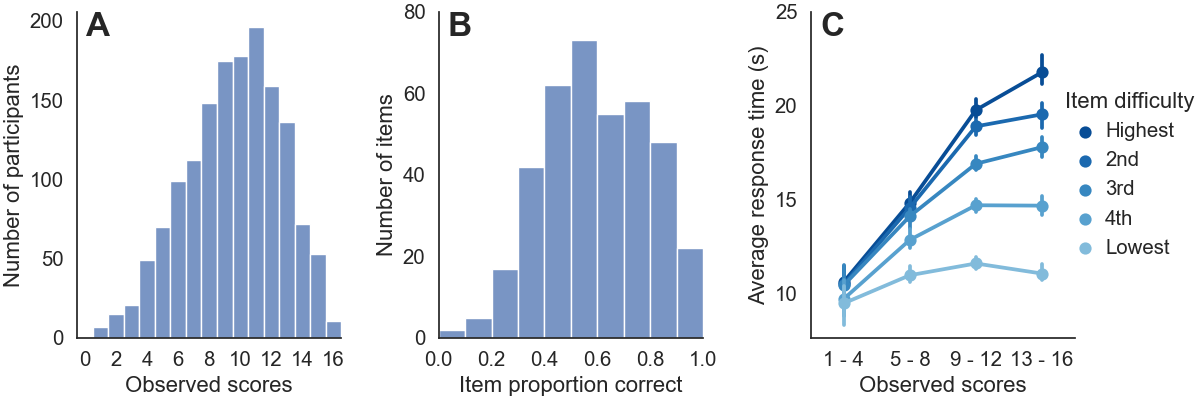
\includegraphics[width=1.0\textwidth]{figures/fig01.png}
\caption{\label{fig:fig01}Summary of performance on the MaRs-IB items. (A) The distribution of total scores across all 1501 participants. (B) The distribution of proportion correct responses across all 384 items. (C) The distribution of participants' median response times across items broken down by participants' total scores and item difficulty (one minus proportion correct responses). Error bars indicate bootstrapped 95\% confidence intervals around the mean.}
\end{figure}
 
\subsubsection{Alternative item structure models}

We fit a series of nested IRT models in order to identify the model that best explained participants' response data. The models varied in how item parameters were estimated, with successive models allowing for greater variability in parameters across item templates and clones. Identifying the model that most accurately captures the structure of item parameters is important in the context of item cloning, as improperly modeled variance can result in the biased estimation of item parameters \citep{lathrop2017item}. 

We fit the models in two waves. The first wave was comprised of four models in which the item discrimination parameters were fixed ($\alpha = 1$).\footnote{Note that these models still included a fixed guessing parameter ($\gamma = 0.25$). We also estimated models with no guessing parameters (i.e. one-parameter logistic or Rasch models), but model comparison indicated these models were worse fits to the data (Table SXX).} We did this in order to minimize the number of total models that we would otherwise need to fit (i.e. all permutations of the four models below, applied to item difficulty and discrimination parameters independently). The first four models were as follows:

\begin{itemize}

\item Model 1a: Item difficulty is a function only of template attributes (number of shapes, number of changing relations). In this model, items of equal complexity are psychometrically equivalent as are all item clones.

\item Model 1b: Item difficulty is a function of template attributes and residuals. In this model, items of equal complexity may not be equally difficult, but all clones of an item are still psychometrically equivalent.

\item Model 1c: Item difficulty is a function of both template and clone attributes (including distractor type and average response time), and template-level residuals. In this model, item clones may systematically vary in their difficulty as a function of their attributes.  

\item Model 1d: Item difficulty is function of both template/clone attributes and residuals. In this model, neither item templates nor clones are psychometrically equivalent. The degree of nonequivalence is dependent on the magnitude of the residual terms.

\end{itemize}

The goodness-of-fit of the four models is summarized in Table \ref{table:1}. Model 1d demonstrated a better fit of the data than Model 1a ($\Delta$ LOCO = 1223.69, se = 44.94), Model 1b ($\Delta$ LOCO 511.58, se = 28.77), and Model 1c ($\Delta$ LOCO = 187.96, se = 17.25). Thus, Model 1d was chosen as the starting point for the second wave of model fitting.

Next we estimated a second set of three models in which the item discrimination parameter was a free parameter. For all models, the item difficulty parameters were specified according to Model 1d. The structure of the three models were as follows:

\begin{itemize}

    \item Model 2a: Item discrimination is a function only of both template and clone attributes. Here we include all attributes at once having found that they were all predictive of item difficulty (see below). 
    
    \item Model 2b: Item discrimination is a function of both item attributes and template residuals. In this model, items of equal complexity may not be equally discriminating.
    
    \item Model 2c: the item discrimination parameters were modeled with fixed and random effects at both levels. In this model, neither item templates nor clones are equivalently discriminating. The degree of nonequivalence is dependent on the magnitude of the residual terms. 
    
\end{itemize}

The goodness-of-fit of these models is summarized in Table \ref{table:1}. Notably, we did not find the most complex model (Model 2c) to be the best-fitting model. Although Model 2c was preferred to Model 2a ($\Delta$ LOCO = 2.13, se = 2.04), it was not preferred to Model 2b ($\Delta$ LOCO = -1.44, se = 0.85).
%We note that the authors of the LOO metric recommend that standard errors be at least twice as large as the difference between models to be confident that one model truly provides a better fit.
However, these differences in LOCO values from each model to the next were each within two standard errors of the mean, indicating only weak predictive improvement of Model 2b over the others \citep{vehtari2022cv}. As such we proceed by select Model 2b as the best-fitting model overall, but proceed in discussing it with caution. We also note that Model 2b fit clearly better than Model 1d ($\Delta$ LOCO = 85.91, se = 6.33, supporting the inclusion of varying item discrimination parameters).

\subsubsection{Objective 1}

Across all items, the average item difficulty was $\mu_\beta = 0.177$ (95\% HDI = 0.118 -- 0.238). There was also considerable variance in item difficulty (sd = 1.431, 95\% HDI = 1.370 -- 1.492), the smallest ($\beta$ = -3.704, 95\% HDI = -4.687 -- -2.775) and largest ($\beta$ = 3.497, 95\% HDI = 2.481 -- 4.635) item difficulty parameters spanning a wide range. For an average ability participant, these estimates translate to an expected average accuracy of 58.4\% across all items, and essentially ceiling (floor) performance for the least (most) difficult items. Thus, items in MaRs-IB span a substantial range of difficulty. 

In turn, the average item discrimination was $\mu_\alpha = 1.298$ (95\% HDI = 1.212 - 1.385). Variability in item discrimination was modest in comparison to item difficulty (sd = 0.221, 95\% HDI = 0.121 - 0.322). Item difficulty and discrimination were uncorrelated across items ($\rho$ = -0.060, 95\% HDI = -0.379 - 0.250). Following convention \citep{baker2017basics}, the items in the MaRs-IB exhibited medium ($\alpha \in$ 0.65 - 1.34) to high ($\alpha \in$ 1.35 – 1.69) levels of discrimination and are thus suitable for measuring matrix reasoning ability.

\subsubsection{Objective 2}

Next we inspected the associations between item attributes and parameters. As predicted, a one-unit change in the number of item features was associated with an increase in item difficulty ($\delta_{\beta_1}$ = 0.579, 95\% HDI = 0.389 -- 0.770), or an approximate 10.6\% reduction in accuracy for a participant of average ability. Similarly, a one-unit change in the number of changing relations was also associated with an increase in item difficulty ($\delta_{\beta_2}$ = 0.514, 95\% HDI = 0.378 -- 0.663), or a 9.5\% reduction in accuracy. 

Looking next at the clone-level attributes, there was an unexpected association between distractor type and item difficulty ($\delta_{\beta_3}$ = 1.105, 95\% HDI = 0.940 -- 1.269). That is, all else equal, an item with MD distractors was associated with an expected 19.9\% reduction in accuracy compared to items with PD distractors. Finally, as expected, there was a positive association between mean response time and item difficulty ($\delta_{\beta_4}$ = 0.541, 95\% HDI = 0.414 -- 0.671). 

In contrast, there was only one credible association between an item attribute and item discrimination parameters. A one-unit change in the number of changing relations was associated with a small but credible increase in item discrimination  $\delta_{\alpha_2}$ = 0.020, 95\% HDI = 0.003 -- 0.037). There was no reliable association between item discrimination and the number of item features ($\delta_{\alpha_1}$ = -0.015, 95\% HDI = -0.036 -- 0.008), distractor type  ($\delta_{\alpha_3}$ = -0.029, 95\% HDI = -0.065 -- 0.005), or average response time ($\delta_{\alpha_4}$ = -0.010, 95\% HDI = -0.030 -- 0.009).

\subsubsection{Objective 3}

Finally, we inspected the relative contributions of modeled and unmodeled sources to variability in item functioning. The two modeled item-level attributes, number of features and changing relations, explained approximately 65.5\% of the variance in difficulty across the 64 item templates (or 35.0\% of the variance across all 384 items). In conjunction with distractor type, these three item attributes explained nearly half (48.2\%) of the variance in item difficulty across all 384 items. Nevertheless, there was non-negligible residual variability in item difficulty at the template- and clone-level as evidenced by the comparatively better fit of item structure models including random effects terms at both levels. As such, neither item templates nor clones can be considered exchangeable with respect to difficulty.

By contrast, the three inherent item attributes explained  approximately 39.2\% of the variance in item discrimination across item templates. In contrast to item difficulty, model comparison suggested there was only non-negligible residual variance in item discrimination at the template-level. Indeed, a model that included random effects at the clone-level offered a comparably worse fit. As such, there was not credible evidence that item clones are not exchangeable with respect to discrimination. 

\subsubsection{Person-level effects}

We investigated person-level abilities as a function of four covariates: age, gender, average response time, and $\Delta$ response time. This last term reflects the degree to which a participant slowed down (or sped up) their response time as a function of item difficulty (Figure \ref{fig:fig01}c). All covariates were standard-scored prior to analysis with the exception of gender, which was binary coded (male = -0.5, female = 0.5).

There was a negative association between age and ability ($\rho_1$ = -0.299, 95\% HDI = -0.353 -- -0.246). There was a small but credible association between gender and ability ($\rho_2$ = 0.128, 95\% HDI = 0.078 -- 0.182), such that women performed marginally better than men. Average response time was positively associated with ability ($\rho_3$ = 0.427, 95\% HDI = 0.374 -- 0.478), as was $\Delta$ response time ($\rho_4$ = 0.368, 95\% HDI = 0.313 -- 0.424), indicating a speed-accuracy tradeoff. 

\subsubsection{Model Fit}

Finally, we validated the fit of the winning model using several posterior predictive model checking measures. Across the 384 items, the average posterior predictive p-value for the $S-\chi^2$ index of item fit was $p = 0.510$ (sd = 0.242). Only 14 items (3.64\%) indicated misfit with posterior predictive p-values less than 0.05 or greater than 0.95. Moreover, the posterior predictive p-value for the test of undimensionality was $p = 0.803$. Though this suggests some evidence for local dependence, it is within a tolerable range. Overall then, the best-fitting model provides an adequate fit to the data.

\subsection{Discussion}

In this first study, we recruited a large sample of adults to complete items from the MaRs-IB, making sure that each item (and its variants) were completed by a sizable number of participants. Using hierarchical item response models, we then measured the psychometric properties (i.e. difficulty and discrimination) of each item. Corroborating the initial study from \cite{chierchia2019matrix}, we found that the items of the MaRs-IB vary greatly in their difficulty -- a prerequisite for measuring nonverbal reasoning across the ability spectrum. We also found that the items of the MaRs-IB exhibited medium-to-large levels of discrimination \citep{baker2017basics}, similar to what has been reported in previous item response theory analyses of the Raven's progressive matrices \citep{chiesi2012using}.

Moreover, using item cloning models we were able to test several important properties of the MaRs-IB items. First, we confirmed that item difficulty is a function of and to a moderate extent explained by its attributes (namely, the number of features and the number of changing relations). Relatedly, we identified that an item's discrimination is a function and partially explained by its number of changing relations, which is similar to what has been reported in other investigations of matrix reasoning tasks \citep{embretson1999generating}. Second, we found that item variants are not equivalent and exchangeable with respect to difficulty. Unexpectedly, and contrary to \cite{chierchia2019matrix}, distractor type emerged as a strong predictor of item difficulty. All else being equal, item variants using MD distractors were harder than the same items using PD distractors. Importantly, once taking this (and the residual variance in difficulty at the item family level) into account, a large majority of item difficulty (72.0\%) was accounted for, suggesting that a minority of variance in difficulty across item variants stems from unmodeled features such as their superficial perceptual properties. 

summary sentence here saying that the MaRs-IB has many desirable properties. We next move onto test construction.

\section{Validation Study}

\subsection{Optimal test assembly}

With 64 item templates, with 6 variants each, there is a vast number of possible test forms we could construct using the MaRs-IB. Returning to our motivating problem --- the availability of abbreviated matrix reasoning measures with the potential for retest --- we opted to construct three parallel short form measures. To do so, we used mixed integer programming \citep{der2005wj} to maximize the test information function (TIF) of each short form subject to the following constraints:

\begin{enumerate}

    \item Each short form was required to contain 12 items. This was chosen to minimize the administration time of a given form (2-4 minutes on average) and to achieve good score reliability (Cronbach's $\alpha \geq 0.8$).
    
    \item All short forms were required to be comprised of variants from the same item families. This was chosen to maximize the similarity of the short forms.
    
    \item Variants could be of the MD or PD distractor type, but not both. This was chosen to prevent item redundancy (i.e. including the same puzzle twice in one short form).
    
    \item The difference in TIFs between short forms was required to be minimized. This was chosen to ensure that each short form had similar psychometric properties (i.e. equivalent reliability across ability levels). 
    
\end{enumerate}

\noindent The TIF was maximized at five ability levels ($\theta = -1.0, -0.5, 0.0, 0.5, 1.0$). Previous simulation studies have shown that target values at three to five well-chosen $\theta$s generally suffice \citep{der2005wj}. Solutions to the mixed integer programming problem were found using the \textit{mip} python package (v1.13.0) \citep{santos2020mixed}.

The results of the test assembly are presented in Figure \ref{fig:fig02}. As expected, the MIP solver selected for items that were more discriminating on average (Figure \ref{fig:fig02}a). Though this was not an explicit constraint, the test characteristic curves (TCCs) of the three short forms are markedly similar, each with an expected total score of 7.7 out of 12 items. Note that, because low ability participants are expected to guess an item correctly 25\% of time, the lower asymptote of the expected score distribution is 3 and the total score distribution is left-skewed. Finally, the TIFs across the three short forms are remarkably similar (Figure~\ref{fig:fig02}b) as would be expected given the assembly constraints. As such, the short forms are predicted to have similar levels of precision across ability levels. Indeed, the expected marginal score reliability for each test form are similar (short form 1: $\alpha = 0.794$; short form 2: $\alpha = 0.795$; short form 3: $\alpha = 0.792$). 

\begin{figure}
\centering
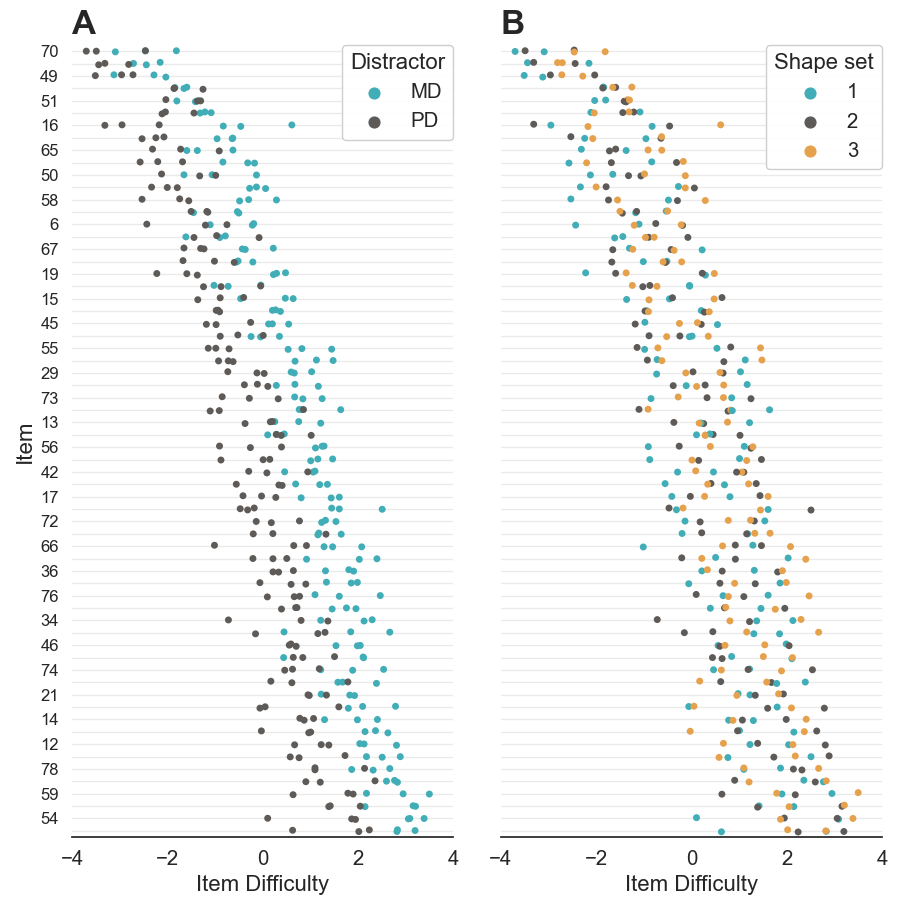
\includegraphics[width=1.0\textwidth]{figures/fig02.png}
\caption{\label{fig:fig02}Results from the test assembly of three parallel MaRs-IB short form (SF) measures. (A) The psychometric properties of the items selected for each form, compared to all remaining items. Points represent the posterior means of the item difficulty and discrimination  parameters. (B) The test characteristic curves (TCCs) for each short form. The degree of overlap highlights the similarity of expected scores for each test form. (C) The test information functions (TIFs) for each short form. The degree of overlap highlights the similarity of reliability for each test form.}
\end{figure}

Next, we proceeded to test each short form in a new sample of participants. The goals for this study were twofold. First, we sought to confirm that each short form would have the properties predicted above. Second, we sought to establish the convergent validity of the short forms by correlating total scores with performance on an abbreviated version of the Raven's progressive matrices.

\subsection{Methods}

\subsubsection{Participants}

A total of N=347 participants were recruited from the Prolific Academic platform (https://www.prolific.co) to participate in an online behavioral experiment in November, 2021. Participants were eligible if they currently resided in the United States and had not participated in the previous study. Total study duration was approximately 10.8 minutes (sd = 4.6) per participant. Participants received monetary compensation for their time (rate USD \$10/hr), plus a performance-based bonus up to \$0.75 based on task performance. Participants earned on average \$2.10 USD (sd = \$0.18 sd). This study was approved by the Institutional Review Board of Princeton University (\#7392), and all participants provided informed consent. 

To ensure data quality, the data from multiple participants were excluded prior to analysis (see Exclusion Criteria below) leaving the data from N=300 participants for analysis. The majority of participants identified as women (men: N=138; women: N=147; non-binary or other: N=13; rather not say: N=2). Participants were 35.0 years old (13.2 sd) on average. The sample was relatively well-educated, with the majority having completed a Bachelor's degree (N=121) or Master's degree or higher (N=45). By comparison, fewer participants endorsed having completed only some college (N=100), only a high school degree (N=33), or preferred not to say (N=1). 

\subsubsection{Procedure}

The study procedure was divided into three sections. After providing consent, participants first completed three short surveys: the 10-item need for cognition survey \citep{chiesi2018applying}, the 8-item PROMIS Cognitive Function-Short Form (8a) \citep{iverson2021normative}, and the 8-item subject numeracy scale \citep{fagerlin2007measuring}. These measures were included as part of exploratory analyses that are reported in the Supplement. Afterwards participants completed one of the three 12-item MaRs-IB short-form measures described above. The administration procedure of the short-forms was identical to that in the first study. Finally, participants completed the 9-item abbreviated Raven's progressive matrices (RPM; form A) \citep{bilker2012development}. The presentation format and instructions for the RPM items was the same as for the MaRs-IB items.

\subsubsection{Exclusion criteria}

To ensure data quality, the data from multiple participants were excluded prior to analysis for one or more of the following reasons: failing to complete all three sections of the experiment (N=17); failing one or more attention checks \citep{zorowitz2021inattentive} embedded in the self-report measures (N=21); experiencing technical difficulties during the experiment (N=11); rapid guessing on four or more items (N=3); or failing to respond on four or more items (N=1). In total, 47 of 347 (13.5\%) participants were excluded leaving the data from N=300 participants for analysis.

\subsubsection{Analysis}

To measure the convergent validity between the MaRs-IB and RPM measures, we fit an additional explanatory item response model. Here participants' ability on the MaRs-IB short forms were estimated as a function of their gender, age, and observed score on the RPM (Eq \ref{eq:4}). The probability of a participant correctly solving a MaRs-IB was defined according to the 3PL model (Eq \ref{eq:1}), where the difficulty and discrimination parameters for an item were fixed to the posterior mean of the estimates obtained in the previous study. Thus, the model estimates the partial correlation between RPM performance and MaRs-IB ability controlling for the age and gender of the participants.

The IRT model was estimated within a Bayesian framework using Hamiltonian Monte Carlo as implemented in Stan (v2.22) \citep{carpenter2017stan}. Four separate chains with randomised start values each took 7500 samples from the posterior. The first 5,000 samples from each chain were discarded. As such, 10,000 post-warmup samples from the joint posterior were retained. The $\hat{R}$ values for all parameters were equal to or less than 1.01, indicating acceptable convergence between chains, and there were no divergent transitions in any chain. 

We calculated the ordinal reliability of the MaRs-IB and RPM short-form measures using the lavaan \citep{lavaan} and semTools \citep{semtools} packages available in R.

\subsection{Results}

Performance on the MaRs-IB short-forms is summarized in Table \ref{table:3}. On average, participants completed the measure in 174 s (sd = 54.0 s) and responded correctly on 8.0 of 12 items (sd = 2.5). The distribution of observed scores was right-shifted (Figure~\ref{fig:fig03}), as was expected given the nominal guessing rate. A one-way ANOVA comparing the average score across the three short-forms was not statistically significant (F(2,297) = 0.253, p = 0.777). Importantly, the ordinal reliability of each measure was satisfactory (all $\alpha > 0.75$). In sum, performance on the MaRs-IB short form were consistent with predicted made during test assembly, indicating that the psychometric properties of the items were adequately calibrated during in the previous study.

Performance on the abbreviated RPM measure is also summarized in Table \ref{table:3}. On average, participants completed the measure in 125 s (sd = 40.1 s) and responded correctly on 4.5 of 9 items (sd = 2.0). The proportion of correct responses on on the RPM was significantly lower than that observed for the MaRs-IB ($t = 13.028$, $p < 0.001$), suggesting that the RPM is more difficult or less biased by guessing.\footnote{In contrast to the MaRs-IB, items in the RPM have either six or eight response options. As such, the nominal guessing rate is expected to be lower for the RPM.} The ordinal reliability for the RPM was also adequate.

The partial correlation between observed scores on the RPM and ability on the MaRs-IB was $\rho = 0.527$ (95\% HDI = 0.457 - 0.577). Considering the attenuation of correlations between two imperfect measures \citep{spearman1961proof}, we should not expect correlations much larger than $\rho = 0.64$ (or $0.80^2$). As such, this result indicates good convergent validity between the two matrix reasoning measures. Briefly, in this smaller sample, neither age nor gender was credibly associated with performance on the MaRs-IB short forms (age: $\rho$ = -0.123, 95\% HDI = -0.253 -- 0.013; gender: $\rho$ = -0.025, 95\% HDI = -0.160 -- 0.108). 

To summarize this section, we used the item parameters estimated as part of the calibration study, and optimal assembly methods, to construct three new MaRs-IB short form measures. As predicted, these measures were quick to administer, had adequate reliability, and good convergent validity with a second matrix reasoning measure. 

\section{General Discussion}

Here we have provided the most comprehensive interrogation of of the MaRs-IB to date. Using item structure models fit to data collected from a large sample of adult participants, we found that the MaRs-IB possesses desirable psychometric properties. The items in the MaRs-IB span a considerable range of difficulty and exhibit medium-to-high levels of discrimination. As such the MaRs-IB is suitable for measuring matrix reasoning across the ability spectrum in the adults. We also verified that the design of the MaRs-IB was in part successful: as intended, item attributes such as feature number and rule number were positively associated with, and explained much of the variability, in item difficulty. Contrary to our expectations, however, we also found that the design of the MaRs-IB had unintended consequences: distractor type was also associated with item difficulty. Moreover, we found non-negligible variability in the difficulty of item clones even after controlling for distractor type. Crucially, item clones in the MaRs-IB therefore cannot be treated as exchangeable. 

With the estimated item parameters, we then constructed three new MaRs-IB short-form measures using optimal test assembly methods. These abbreviated test measures were designed to measure matrix reasoning ability with maximal reliability in the general adult population under several desirable constraints (i.e. 12 item limit, administration time of 2-4 minutes). In a second sample of participants, we found that each short form measure had adequate reliability (Cronbach $\alpha \approx 0.8$) and good convergent validity with an abbreviated Raven's progressive matrices measure. Moreover, the observed scores on the short-forms followed the expected distribution as predicted by their test characteristic curves. These results demonstrate the success of the item calibration study in producing accurate estimates of the item parameters. 

Of additional note are the associations we found between accuracy and response time. The best-performing participants spent more time on each item, consistent with a speed-accuracy trade-off account of performance \citep{heitz2014speed}. Interestingly, we also found an interaction between participant ability and item difficulty; that is, the best-performing participants increased their deliberation time as items become more difficult, whereas the worst-performing participants maintained approximately the same work rate. These results are consistent with a persistence account of participant ability, wherein performance reflects in part a willingness to invest time in the solution process \citep{ranger2021effects}. As such, the MaRs-IB may be suitable not only for measuring matrix reasoning ability but also mental effort costs [cite], opportunity costs [cite], or other  motivational factors \citep{duckworth2011role} related to the tendency to give up (at least in low-stakes test settings; see \cite{shaw2020reasoning} for a counter-example). Moreover, the use of cognitive models may help to disentangle the relative contributions of these factors to performance on the MaRs-IB \citep{ranger2014accumulator}.

The current investigation of the MaRs-IB is not without its own limitations. One notable limitation is our sample. Here we analyzed response data collected from an online, adult sample that was relatively young and well-educated. We cannot guarantee that the psychometric properties of the MaRs-IB reported here will generalize to other populations or testing contexts. Future researchers may consider replicating the current study in other populations of interest (e.g. children, clinical samples). By using item response models here, however, we make possible the opportunity for future IRT ``linking'' studies. IRT linking describes a set of methods to establish the comparability of item and ability parameters estimated from data collected from two or more groups that differ in ability \citep{lee2018irt}. Future studies employing these methods could provide insight not only in how the functioning of the MaRs-IB may change in different populations, but also how matrix reasoning ability differs across samples.

A second limitation is in our investigation of sources of variance. Here we only investigated the contributions of three item attributes. There are far more sources to have investigated (e.g. type of rule change such as color change versus shape change). Indeed, there are other item features taxonomies we could have explored \citep{carpenter1990one}. We also did not explicitly model perceptual features as has been done before. Although doing so would not change our results about exchangeability of item clones, it would allow for more precise estimates of item parameters and improved test assembly. Also allows for possibility of automatic item generation. Room for future research. 

In summary, we have provided an in-depth psychometric validation of the MaRs-IB, finding that it is suitable for measuring matrix reasoning ability in the general adult population. We release the item parameters so that researchers interested in measuring matrix reasoning can construct maximally reliable tests for their own research.

\bibliography{references}

\begin{table}[]
\centering
\begin{tabular*}{\textwidth}{lc@{\hskip 6mm}r@{\hskip 6mm}c}
\toprule
Predictor &  Coef. (SE) & Z-score (p-value) & 95\% CI  \\
\midrule
Accuracy & 0.039 (0.007) &   5.367 (<0.001) &  0.025 -- 0.053  \\
Score &  0.167 (0.009) &  19.204 (<0.001) &  0.150 -- 0.184  \\
Difficulty & 0.073 (0.005) &  13.292 (<0.001) &  0.062 -- 0.083  \\
Accuracy x Score & -0.064 (0.007) &  -8.764 (<0.001) & -0.078 -- -0.050  \\
Accuracy x Difficulty & 0.097 (0.007) &  14.351 (<0.001) &  0.084 -- 0.110  \\
Score x Difficulty &  0.032 (0.005) &   6.549 (<0.001) &  0.023 -- 0.042  \\
Accuracy x Score x Difficulty &  0.012 (0.006) & 1.955 (0.051) & -0.000 -- 0.025  \\
\bottomrule
\end{tabular*}
\caption{\label{table:1}\normalfont Summary of the random-intercepts linear regression model predicting log-transformed response time as a function of accuracy, participant rest score, and item difficulty.}
\end{table}

\begin{table}
    \centering
    \begin{tabular*}{\textwidth}{cccccccc}
    \toprule
    Model & FE-1 & RE-1 & FE-2 & RE-2 & psis-loco & $\Delta$ psis-loco (se) \\
    \midrule
    1a & x &   &   &   & -14516.85 & -1223.69 (44.94)\\
    1b & x & x &   &   & -13804.74 & -511.58 (28.77) \\
    1c & x & x & x &   & -13481.12 & -187.96 (17.25) \\
    1d & x & x & x & x & -13293.16 & - \\
    \midrule
    2a & x &   & x &   & -13209.38 & -2.13 (2.04) \\
    2b & x & x & x &   & -13207.25 & - \\
    2c & x & x & x & x & -13208.69 & 1.44 (0.85) \\
    \bottomrule
    \end{tabular*}
    \caption{\label{tab:2} \normalfont Goodness of fit of item response models to MaRs-IB data. Pareto-smoothed importance sampling}
    \label{table:2}
\end{table}

\begin{table}
    \centering
    \begin{tabular*}{\textwidth}{lccccc}
    \toprule
    Measure & Sample & Task Time (sd) & Mean Score (sd) & IQR & Reliability ($\alpha$) \\
    \midrule
    MaRs-IB SF-1 & 103 & 174.9 s (53.3) & 7.9 (2.4) & 7 - 10 & 0.761 \\
    MaRs-IB SF-2 & 98  & 169.0 s (53.0) & 8.2 (2.6) & 7 - 10 & 0.810 \\
    MaRs-IB SF-3 & 99  & 178.5 s (55.7) & 7.9 (2.7) & 6 - 10 & 0.829 \\
    RPM SF-A     & 300 & 124.6 s (40.1) & 4.5 (2.0) & 3 - 9 & 0.791 \\
    \bottomrule
    \end{tabular*}
    \caption{\label{table:3} \normalfont Summary of performance on the MaRs-IB and Raven's progressive matrices (RPM) short form (SF) measures. IQR = interquartile range.}
\end{table}

\begin{figure}
\centering
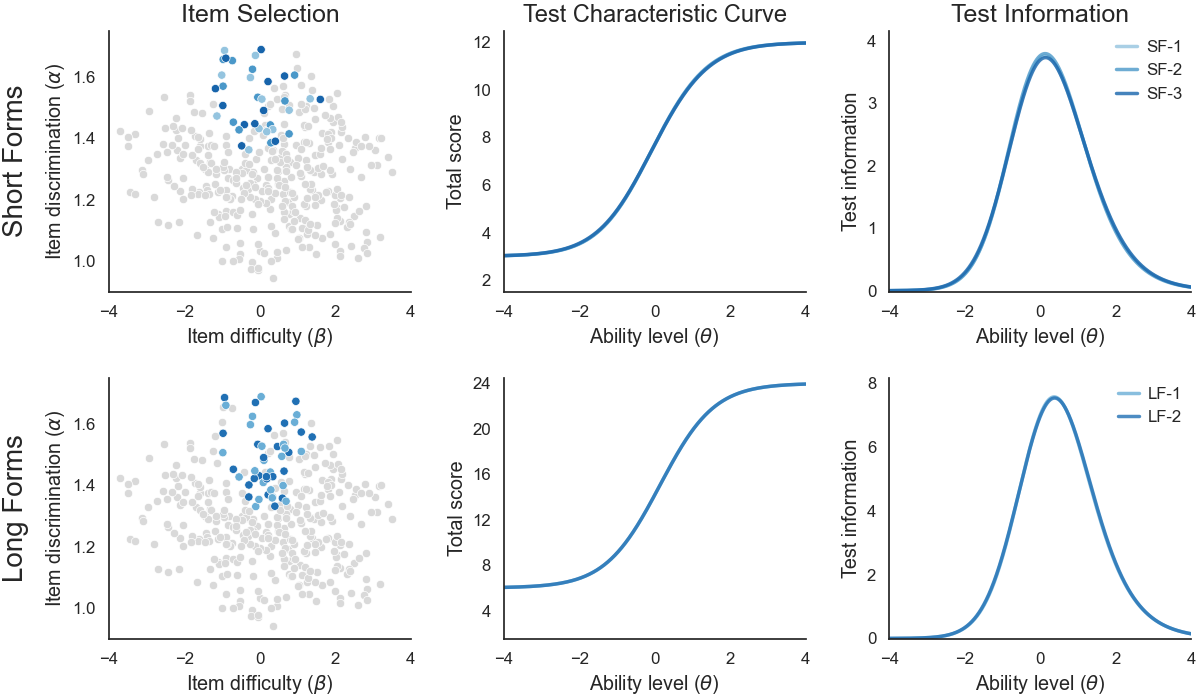
\includegraphics[width=1.0\textwidth]{figures/fig03.png}
\caption{\label{fig:fig03}The joint distribution of total scores on the MaRs-IB short form and abbreviated Raven's progressive matrices (RPM) measures. The distribution of observed scores for each measure are shown in the margins.}
\end{figure}

\end{document}
